\chapter{Proposed Solution and Work Plan} \label{chap:ch4}
\paragraph{}
This chapter presents a preliminary solution to the addressed problem in Section~\ref{sec:proposed_solution} and outlines the corresponding work plan in Section~\ref{sec:work_plan}. Together, these elements define the scope and direction of the work to be carried out in the dissertation.

\section{Preliminary Solution} \label{sec:proposed_solution}
\paragraph{}

This chapter presents a preliminary solution concept for addressing the limitations identified in sequential TEA*-based multi-agent path planning.

The proposed solution builds upon the centralized planning framework previously described and focuses on extending the existing path planner through parallel exploration of agent priority orderings. Figure~\ref{fig:preliminary_solution_scheme} provides a conceptual overview of the proposed approach and highlights its main processing stages.

\begin{figure}[H]
    \centering
    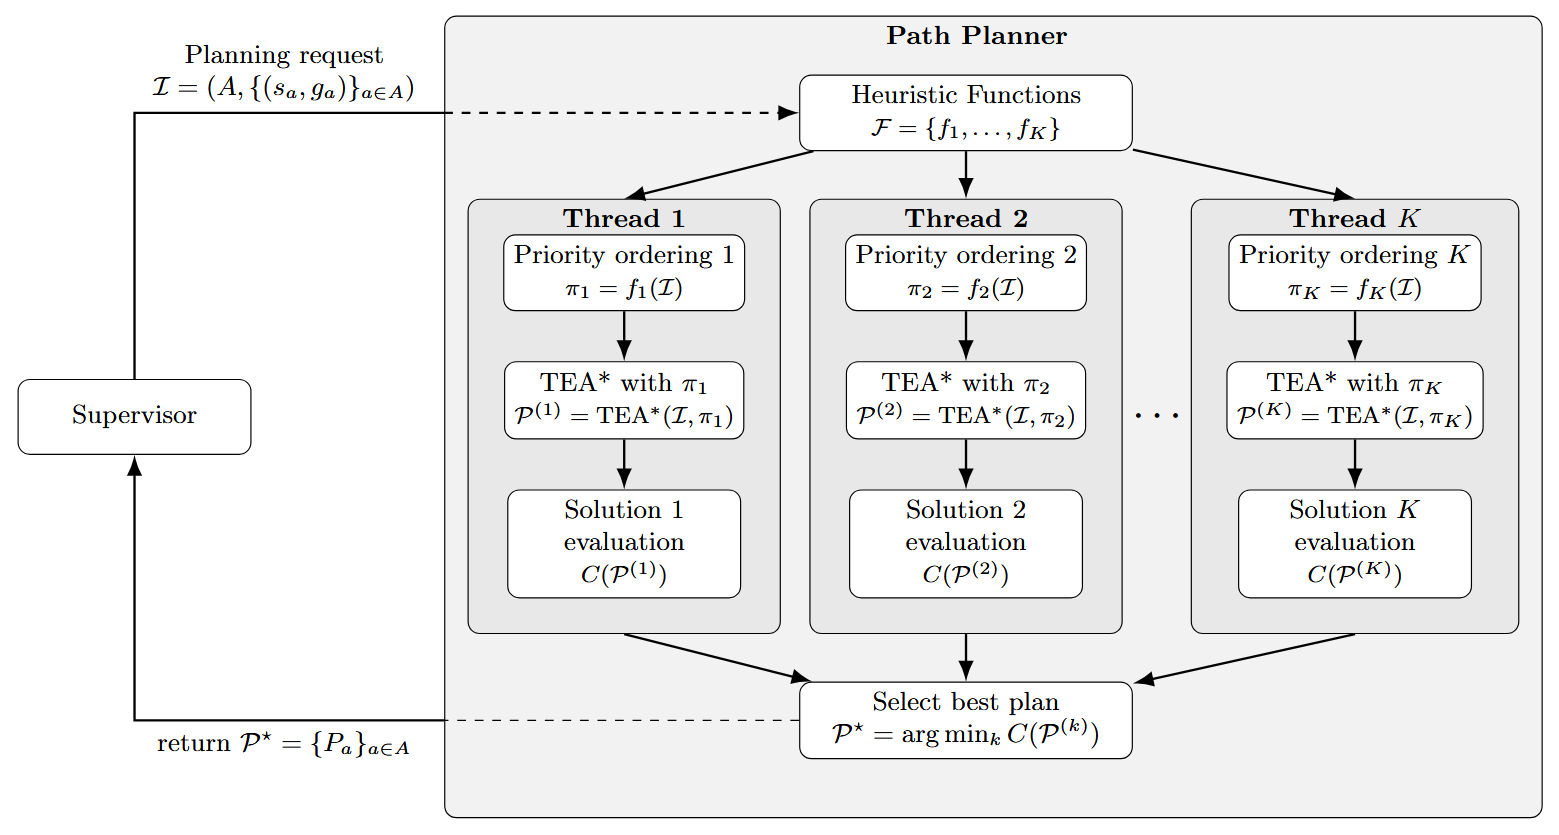
\includegraphics[width=\linewidth]{preliminar_solution_scheme.png}
    \caption{Conceptual overview of the proposed preliminary multithreaded planning approach.}
    \label{fig:preliminary_solution_scheme}
\end{figure}

At a high level, the Supervisor initiates a planning request by providing a set of agents and the respective start and goal vertexes,
$\mathcal{I} = \bigl(A, \{(s_a, g_a)\}_{a \in A}\bigr),
$
where each agent \(a \in A\) is associated with a start vertex \(s_a\) and a goal vertex \(g_a\).

As illustrated in Figure~\ref{fig:preliminary_solution_scheme}, the Path Planner internally relies on a set of heuristic functions
$
\mathcal{F} = \{f_1, \dots, f_K\}
$
to generate multiple priority orderings of the agents. Each heuristic \(f_k\) produces a permutation 
$
\pi_k = f_k(\mathcal{I})
$
, which defines the order in which agents are planned by a sequential TEA* instance. The key idea is that different orderings may lead to substantially different solutions, particularly in constrained environments where resource contention is significant.

Each priority ordering \(\pi_k\) is processed independently within a dedicated planning thread. Inside each thread, the TEA* algorithm is executed sequentially according to the corresponding ordering, yielding a candidate solution
$
\mathcal{P}^{(k)} = \mathrm{TEA}^\ast(\mathcal{I}, \pi_k),
$
where \(\mathcal{P}^{(k)}\) denotes a complete set of trajectories, one per agent. Although TEA* remains sequential within each thread, the overall planning process benefits from parallelism by exploring multiple orderings concurrently, as depicted in the parallel branches of Figure~\ref{fig:preliminary_solution_scheme}.

Following the generation of candidate solutions, each solution is evaluated using a predefined cost function \(C(\cdot)\), which may account for criteria such as makespan, total path cost, or feasibility under temporal constraints. The final output of the Path Planner is obtained by selecting the solution that minimizes the chosen cost metric:
$
\mathcal{P}^\star = \arg\min_k C(\mathcal{P}^{(k)}).
$
The selected plan \(\mathcal{P}^\star = \{P_a\}_{a \in A}\), consisting of one trajectory per agent, is then returned to the Supervisor for execution or further coordination. By leveraging parallel computation to evaluate multiple priority orderings within the same planning time, this preliminary approach aims to improve robustness and solution quality while remaining compatible with the existing centralized planning architecture.

It is worth noting that alternative execution strategies may be considered within this preliminary framework. While the approach illustrated in Figure~\ref{fig:preliminary_solution_scheme} assumes that all parallel planning threads are executed to completion before selecting the best solution, other synchronization policies are possible. In particular, the planning process may be configured to wait for only a subset of the parallel threads to complete before selecting a solution, or to terminate after a predefined time budget and return the best solution found so far.

Such a policy can be controlled through a parameter $\epsilon$, representing the number of completed planning threads required prior to solution selection, with $1 \leq \epsilon \leq K$. Larger values of $\epsilon$ increase confidence that the selected solution is close to the best among the explored orderings, at the cost of higher planning latency, while smaller values favor faster response times with potentially reduced solution quality. This trade-off is also shaped by the characteristics of the employed heuristics, as simpler heuristics may generate solutions more quickly and thus dominate under early termination policies, whereas increasing $\epsilon$ enables broader exploration, including orderings induced by more computationally demanding heuristics. Since higher heuristic complexity does not necessarily imply better solution quality, $\epsilon$ effectively acts as a tuning parameter balancing exploration depth and planning latency. The practical impact of this mechanism is left for future investigation during the implementation and experimental phases of this dissertation.


\section{Work Plan} \label{sec:work_plan}
\paragraph{}

This section outlines the planned timeline for completing the objectives of this dissertation, following a structured, phase-based approach to guide the design, implementation, and evaluation of the proposed multithreaded planning solution.

The work is organized into a set of core tasks addressing the main technical objectives, complemented by a cross-cutting assessment activity that supports optional extensions:

\begin{itemize}
    \item \textbf{Task 1: Environment Setup and Validation (3 weeks).} Configuration and validation of the simulation environment and baseline planner.
    
    \item \textbf{Task 2: Multithreaded TEA* Integration  (3 weeks).} Integration of multithreading mechanisms into the existing TEA*-based planner.
    
    \item \textbf{Task 3: Continuous Assessment of CBSH-RTC Applicability (6 weeks).} Ongoing evaluation of the relevance of CBSH-RTC as a comparative baseline.
    
    \item \textbf{Task 4: Heuristic Design and Integration  (4 weeks).} Design and integration of heuristic strategies for generating diverse agent priority orderings.
    
    \item \textbf{Task 5: Experimental Evaluation (4 weeks).} Definition of evaluation scenarios and systematic assessment of solution quality and computational performance.
    
    \item \textbf{Task 6: Dissertation Writing  (4 weeks).} Consolidation of results and preparation of the final document.
    
\end{itemize}

The work plan is centered on a main development milestone corresponding to the completion and validation of the proposed planner. Optional activities, namely the integration of CBSH-RTC into the centralized fleet coordination framework and its subsequent experimental evaluation, may be pursued depending on the outcome of the assessment task, but are not critical to the successful completion of the dissertation. Figure~\ref{fig:gantt_workplan} presents a graphical overview of the work plan.


\begin{figure}[H]
    \centering
    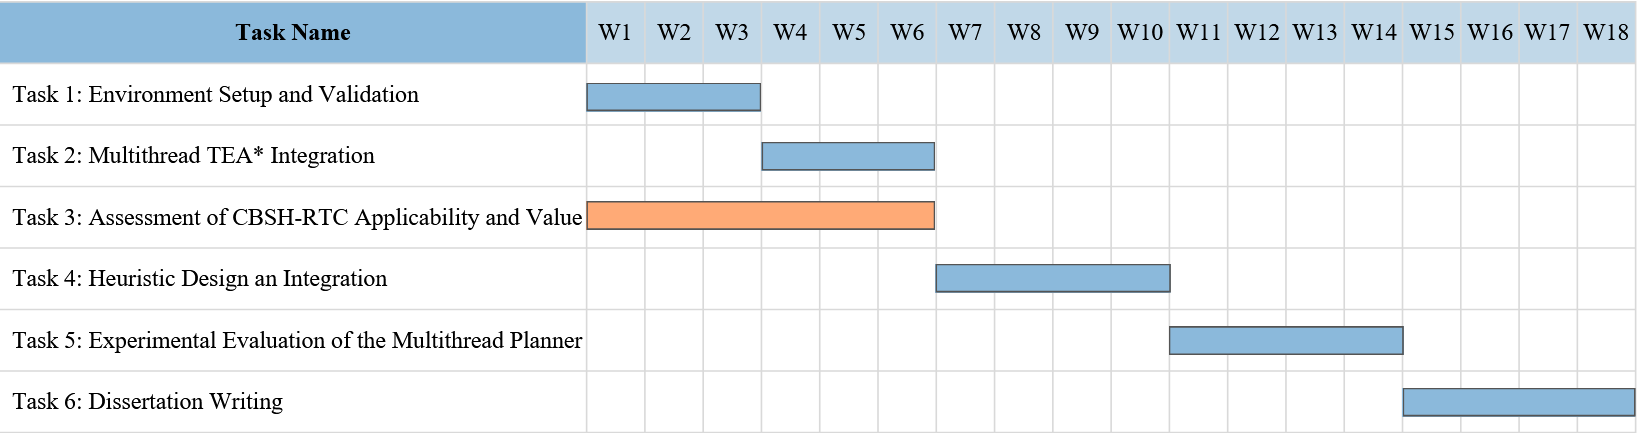
\includegraphics[width=\linewidth]{gantt.png}
    \caption{Gantt chart illustrating the proposed work plan.}
    \label{fig:gantt_workplan}
\end{figure}
